\documentclass[a4paper,12pt]{article}

% Pakete für zusätzliche Funktionen
\usepackage[utf8]{inputenc}   % UTF-8 Zeichencodierung
\usepackage[T1]{fontenc}     % Korrekte Silbentrennung und Umlaute
\usepackage[ngerman]{babel}  % Deutsche Spracheinstellungen
\usepackage{amsmath, amssymb} % Mathematische Symbole
\usepackage{graphicx}        % Einfügen von Bildern
\usepackage{hyperref}        % Hyperlinks
\usepackage{geometry}        % Seitenränder
\usepackage{listings}        % Code-Listings
\usepackage{csquotes}        % Zitate
\usepackage{csvsimple}  % Für das Einfügen von CSV-Dateien
\usepackage{titlesec}
\usepackage{float}  % Add this to your preamble
\newcommand{\sectionbreak}{\clearpage}
\geometry{a4paper, margin=2.5cm}
% Einstellungen für Hyperlinks
\hypersetup{
    colorlinks=true,
    linkcolor=blue,
    citecolor=blue,
    filecolor=magenta,
    urlcolor=cyan,
    pdftitle={Implementierung digitaler Geschäftsprozesse},
    pdfpagemode=FullScreen,
}

% Titel und Autoreninformationen
\title{\textbf{Implementierung digitaler Geschäftsprozesse}}
\author{Kürsat Darcan | MFWS422A}
\date{Abgabedatum: \today}

\begin{document}

% Deckblatt
\maketitle
\thispagestyle{empty}
\vspace{2cm}
\begin{center}
    \includegraphics[width=0.3\textwidth]{FHDW_Logo_RGB-01.svg.png} % Ersetzen Sie "example-image" durch Ihr Logo/Bild
    \\
    \vspace{1cm}
    \textbf{Studiengang: Wirtschaftsinformatik}\\
    \textbf{Fachhochschule der Wirtschaft (FHDW)}
\end{center}
\newpage

% Inhaltsverzeichnis
\renewcommand{\thepage}{\roman{page}} % Seitenzahlen in römischen Ziffern für Verzeichnisse
\tableofcontents
\newpage

% Bei Bedarf Abbildungsverzeichnis
\listoffigures
\addcontentsline{toc}{section}{Abbildungsverzeichnis}
\newpage

% Bei Bedarf Tabellenverzeichnis
\listoftables
\addcontentsline{toc}{section}{Tabellenverzeichnis}
\newpage
%-- Beispiel für eine Tabelle --%
%\begin{table}[htbp]
%    \centering
%    \resizebox{\textwidth}{!}{ 
%    \csvautotabular[separator=semicolon]{tabellen/scm1/test.csv}  % Pfad zur CSV-Datei
%    }
%    \caption{Beispieltabelle aus test.csv}
%    \label{tab:testcsv}
%\end{table}
%-- Ende Beispiel --%

% Abkürzungsverzeichnis
\section*{Abkürzungsverzeichnis}
\addcontentsline{toc}{section}{Abkürzungsverzeichnis}
\begin{description}
    \item[CRM] Customer Relationship Management
    \item[SCM] Supply Chain Management
\end{description}
\newpage

% Hauptteil mit arabischen Seitenzahlen
\renewcommand{\thepage}{\arabic{page}} % Seitenzahlen in arabischen Ziffern für den Hauptteil
\setcounter{page}{1}


% Einleitung
\section{Einleitung}
\subsection{Zielsetzung der Ausarbeitung}
Diese Ausarbeitung ist Teil des Moduls \textbf{Implementierung digitaler Geschäftsprozesse}.
Die Ausarbeitung bildet den Ablauf und die Reflexion des Planspiels \textit{kdibisglobal} ab,
das im Rahmen des Moduls durchgeführt wurde.
Hierbei wird auf die einzelnen Spielrunden eingegangen
und die jeweiligen Ergebnisse und Erkenntnisse analysiert und reflektiert.
Zusätzlich werden weitere Methoden
erläutert, die im Rahmen des Moduls behandelt wurden, aber nicht im Planspiel angewendet werden konnten.

\subsection{Überblick über das Planspiel kdibisglobal}
\textbf{kdibisglobal} wurde speziell für das Buch Integrierte Business-Informationssysteme von Herrn Klaus-Dieter Gronwald entwickelt,
um ein praktisches Verständnis für digitale Geschäftsprozesse zu erlangen.
Das Planspiel simuliert das Geschäftsprozessmanagement für einen Bierhersteller.

In diesem Planspiel übernehmen die Teilnehmer einzelne Bereiche innerhalb des Unternehmens und sind für die jeweiligen Bestellungen zuständig.
Dabei müssen verschiedene Faktoren berücksichtigt werden, wie Lieferverzögerungen, Verfügbarkeit von Produkten, saisonale Nachfrage und so weiter.
Zusätzlich werden wichtige Bereiche wie Supply Chain Management (SCM) und Customer Relationship Management (CRM) abgebildet.

Im Rahmen des SCM geht es darum, Bestände sinnvoll zu planen, Nachbestellungen rechtzeitig auszulösen und Lieferengpässe zu vermeiden.
Beim CRM steht die Beziehung zum Kunden im Vordergrund, also etwa das Management von Aufträgen,
die Sicherstellung einer hohen Kundenzufriedenheit sowie die Reaktion auf Änderungen in der Nachfrage.

Ziel ist es, durch den richtigen Einsatz digitaler Systeme die Unternehmensprozesse effizient zu gestalten.\cite{Kdibisglobal}

% Ablauf und Reflexion des Planspiels
\section{Ablauf und Reflexion des Planspiels}
Die Erkenntnisse sowie die Ergebnisse des Planspiels werden in drei Spielrunden unterteilt und analysiert.
Zusätzlich werden die theoretischen Inhalte aus dem Modul Implementierung digitaler Geschäftsprozesse erläutert und
in den Kontext des Planspiels gesetzt.

Für die Spielrunden SCM1 und SCM2 wird das Supply Chain Management nur im Bereich des Einzelhandels betrachtet,
da der Autor der Ausarbeitung hierfür zuständig war.

Für die Spielrunde CRM2 wird das Customer Relationship Management betrachtet. Da jedes Teammitglied einen Einzelhandel repräsentiert hat, also 5 Teammitglieder auf 4 Einzelhandel verteilt wurden,
mussten der Autor und ein weiteres Teammitglied gemeinsam für Einzelhandel 1 agieren. Jeder Einzelhandel hatte bis zu 11 Produkte. Da in Einzelhandel 1 zwei Teammitglieder zuständig waren, mussten die Produkte durch 2 aufgeteilt werden.
Dem entsprechend kann nicht das gesamte Einzelhandelsproduktsortiment betrachtet werden, sondern nur die Produkte, für die der Autor zuständig war.

\subsection{Spielrunde 1 – SCM1: Bullwhip Game und ERP-Strategie}
SCM 1 ist die erste Spielrunde, in dem ein Jahr simuliert wird unnd eine Bestellzyklus von 1 Woche besteht, was 52 Spielrunden entspricht.
Zudem gibt es in diesem Spieljahr keinen Forecast, kein Inventory Management und keine Kommunikation zwischen den Teammitglieder.
Ziel ist es dabei die Auswirkungen eines nicht kommunikativen Supply Chain Management zu erfahren und eine Demonstration des Bullwhip-Effekts zu erfahren.
--Quelle--

Nachdem die  erste spielrunde erläuert wurde, wird auf die einzelnen Spielrunden eingegangen.
%\begin{table}[H]
%    \centering
%    \resizebox{\textwidth}{!}{ 
%    \csvautotabular[separator=semicolon]{tabellen/scm1/scm1komplettablauf.csv}  % Pfad zur CSV-Datei
%    }
%    \caption{SCM 1 Spielablauf}
%    \label{tab:SCM 1 Spielablauf}
%\end{table}

Wie aus der Tabelle zu entnehmen ist, verliefen die ersten 10 Spielrunden sehr erfolgreich, und die Bestellungen wurden stets rechtzeitig ausgelöst.
Zusätzlich konnte die Lagerhaltung konstant bei durchschnittlich 1000 hl gehalten werden.

Ab Woche 11 kam es jedoch zu plötzlichen Lieferverzögerungen, die durch die Simulation verursacht wurden.
Trotz der Regeln des Planspiels ließ sich die Ursache der Verzögerungen nicht feststellen, da zu diesem Zeitpunkt keine Kommunikation zwischen den Teammitgliedern stattfinden konnte.
Infolge der Lieferprobleme konnten die Bestellungen an die Einzelhändler nicht vollständig ausgeliefert werden, wodurch bis Woche 14 Fehlmengen von bis zu 9000 hl auftraten.

Zudem führte Unerfahrenheit zu mehreren Überbestellungen in den Wochen 13 und 14.
Hätte sich die Überbestellung nur auf Woche 13 beschränkt, wären die Auswirkungen auf die Lagerhaltung gering gewesen,
da dadurch die Fehlmengen der Wochen 12 bis 14 ausgeglichen worden wären und ein Lagerbestand von über 4000 hl erzielt worden wäre.
Die zusätzlichen Bestellungen in Woche 14 bewirkten jedoch, dass der Lagerbestand in Woche 17 auf über 15000 hl anwuchs.
Dies verursachte hohe Lagerkosten, die erst bis Woche 23 durch den Bestelleingang teilweise ausgeglichen werden konnten.
In diesem Zeitraum kam es zu Bestellungen mit weniger als 1000 hl, wodurch der Bullwhip-Effekt deutlich erkennbar wurde.

Fehlkalkulationen und der Bullwhip-Effekt führten zu emotionalen Reaktionen: Lagerbestände sowie Bestell- und Auslieferungsprozesse wurden zunehmend unachtsam gehandhabt.
In den Wochen 24 bis 26 entstanden dadurch weitere Fehlmengen, die aufgrund unüberlegter Bestellungen nicht mehr ausgeglichen werden konnten.

Zwischen Woche 26 und Woche 36 stabilisierte sich die Situation, und Lagerbestände sowie Bestellungen konnten wieder besser aufeinander abgestimmt werden.

In den Wochen 37 bis 52 bestand das Ziel darin, Fehlmengen zu vermeiden und stets einen ausreichenden Lagerbestand vorzuhalten,
um vollständige Auslieferungen zu gewährleisten.
Allerdings führte dieses Ziel zu erneut hohen Lagerkosten, verursacht durch Überbestellungen im Verlauf der Wochen ab Woche 37.
Auch hier kam es wieder zu emotional gesteuerten Bestellungen, die ohne sorgfältige Berücksichtigung des tatsächlichen Bestelleingangs ausgelöst wurden, lediglich um Fehlmengen zu verhindern.

%\begin{figure}[H]
%    \centering
%    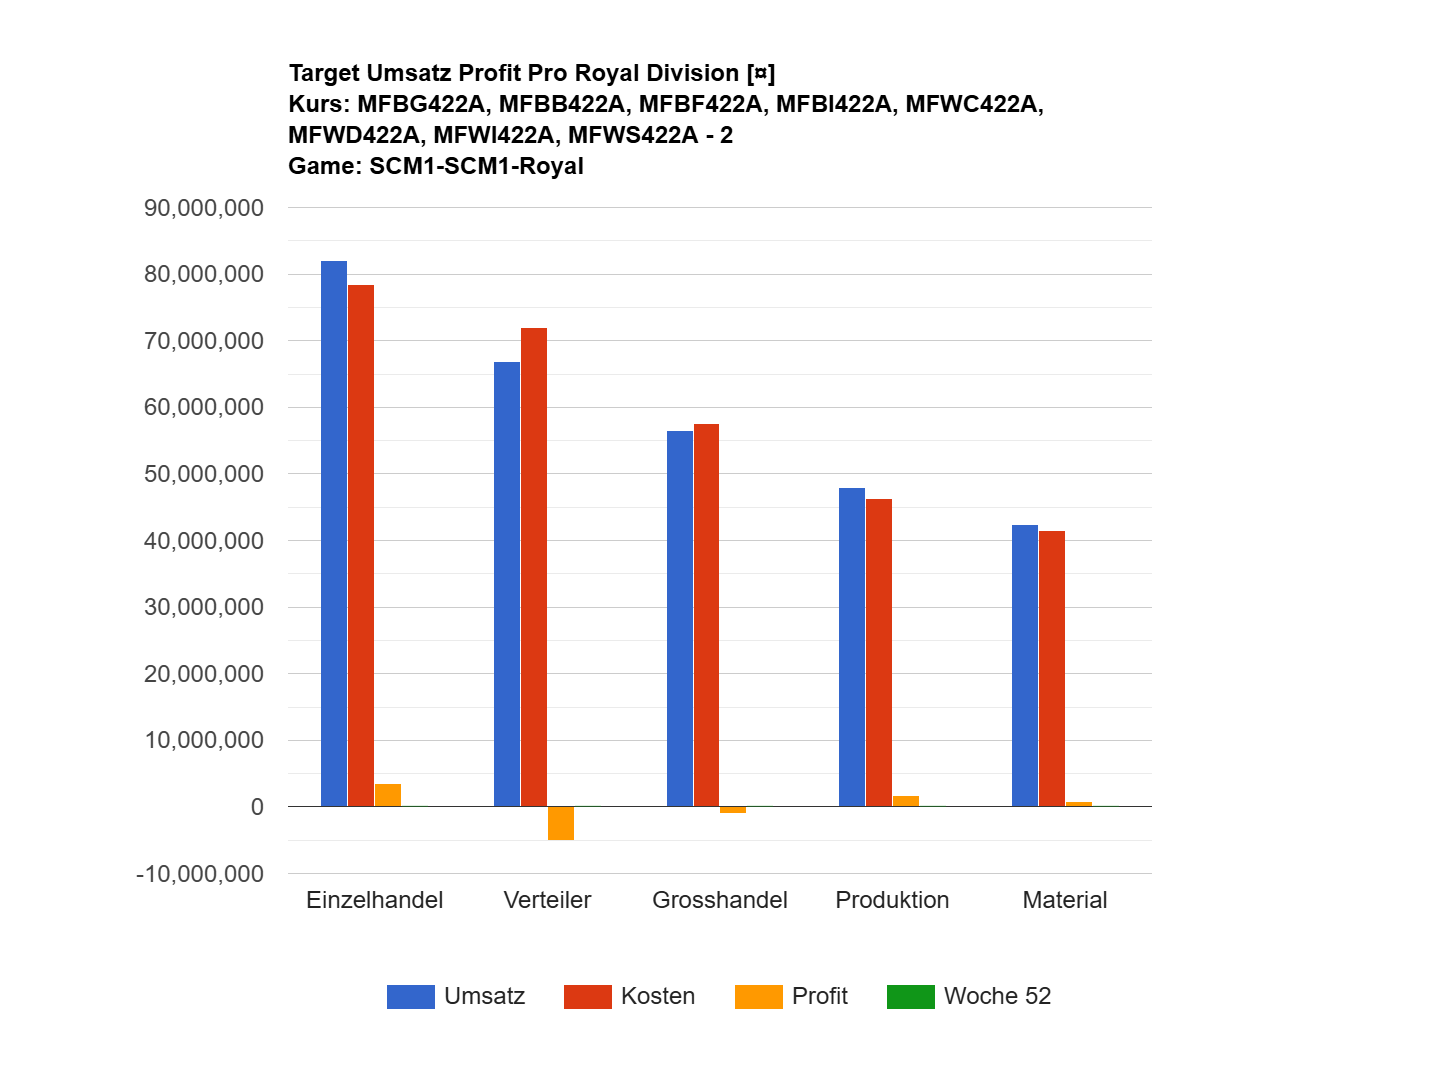
\includegraphics[width=0.7\textwidth]{abbildungen/scm1/scm1Umsatz.png}
%    \caption{SCM1 Umsatz}
%    \label{fig:SCM1 Umsatz}
%\end{figure}

Dennoch ist deutlich anhand des Abbilds zu erkennen, dass die Umsätze für den Einzelhandel mehr als 3,5 Millionen Euro betrugen
und der Bullwhip-Effekt keinen großen Einfluss auf den Umsatz hatte, wie in den anderen Unternehmensbereichen.

\subsubsection{Ursachen des Bullwhip-Effekts im Planspiel}
Nun wurde mehr mals erwähnt, dass der Bullwhip-Effekt aufgetreten ist.
Was genau bedeuetet den Bullwhip-Effekt, wie kommt dieser zustande und wie kann dieser vermieden werden?
%\begin{figure}[H]
%    \centering
%    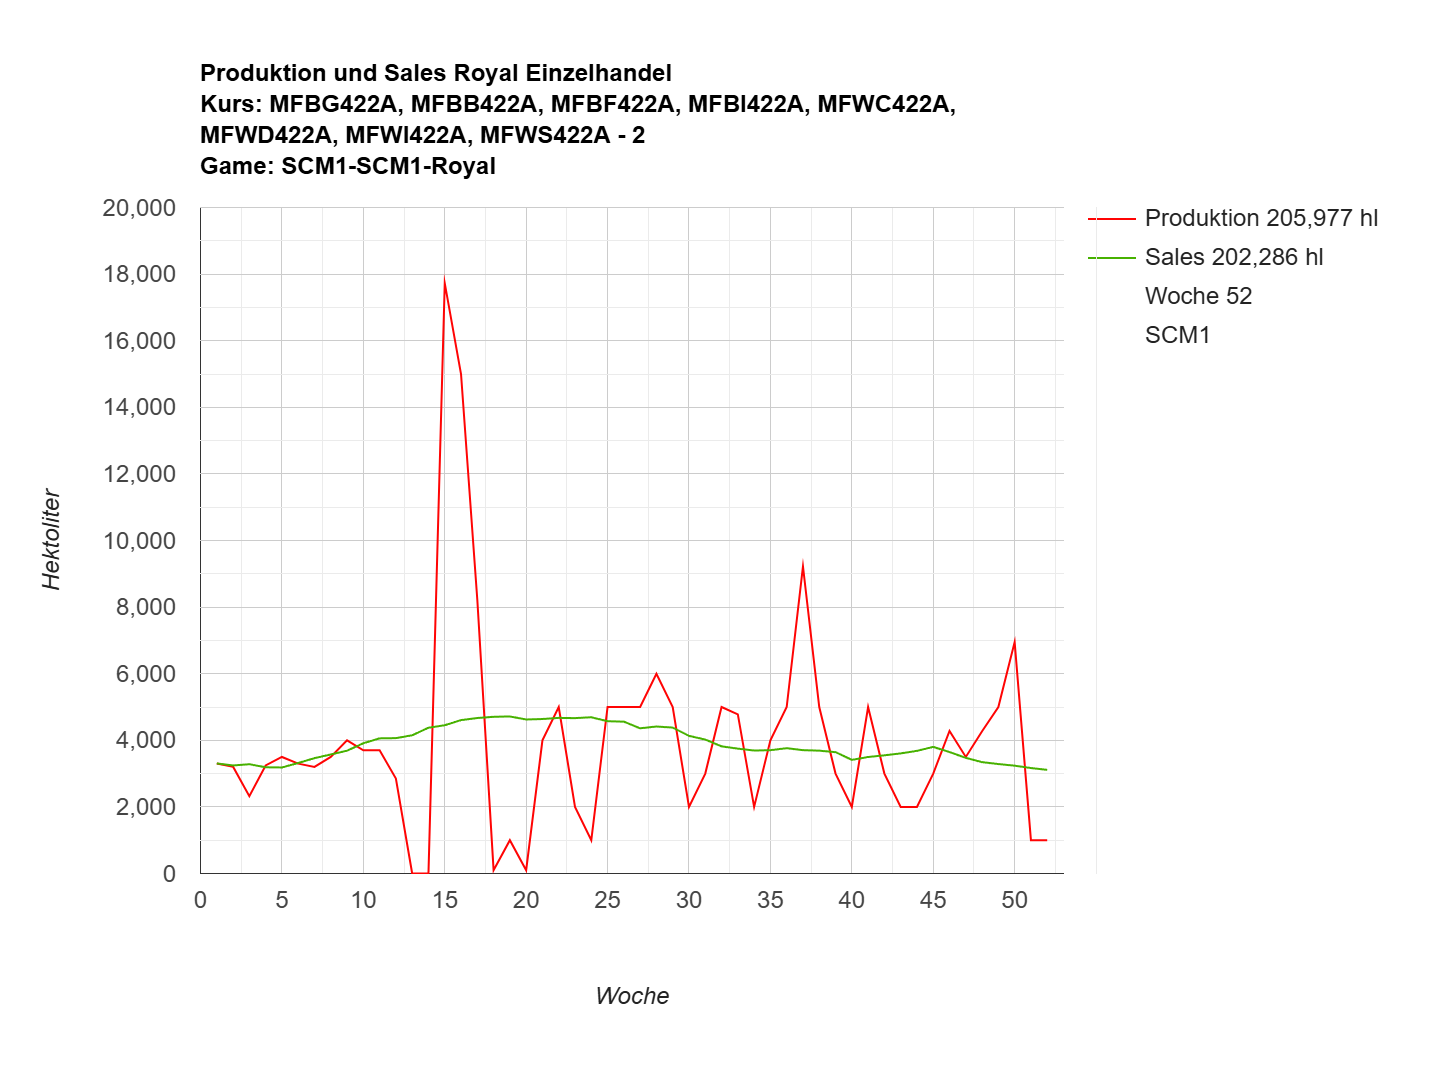
\includegraphics[width=0.7\textwidth]{abbildungen/scm1/scm1bullwhipeffektindex.png}
%    \caption{SCM1 Bullwhip-Effekt-Index}
%    \label{fig:SCM1 Bullwhip-Effekt-Index}
%\end{figure}
Auch soll die Abbildung \ref{fig:SCM1 Bullwhip-Effekt-Index} verdeutlichen, wie stark der Bullwhip-Effekt ausgeprägt sein kann.
Wie setzt sich der Bullwhip-Effekt zusammen? Zum einen, wie in Kapitel Spielrunde 1 erläutert, liegt es an mangelnder Kommunikation zwischen den Teammitgliedern,
 zum anderen an fehlender Transparenz zwischen den Bereichen.
Zudem spielen weitere Faktoren eine Rolle, wie zum Beispiel Demand Signal Processing, das bei saisonaler Nachfrage zu Überreaktionen oder Fehleinschätzungen führen kann.
Auch Order Batching oder eine lange Lead Time können den Bullwhip-Effekt deutlich verstärken.
Das bedeutet: Wenn Abteilungen Bestellungen auf- oder abrunden, kommt es zu stärkeren Verzerrungen der Bestellmengen, die dazu führen können, dass der Bullwhip-Effekt sich erkennbar macht.
Bei der Lead Time spielt die Zeitdifferenz zwischen Bestellung und Erhalt der Ware eine entscheidende Rolle.
Wenn Teammitglieder auf die Supply Chain reagieren, die Waren jedoch verzögert eintreffen, kann ein starker Effekt entstehen, wie es in den Wochen 11–18 aufgetreten ist und in Abbildung \ref{fig:SCM1 Bullwhip-Effekt-Index} erkennbar ist.

\subsubsection{IT-Situation der Einzelhandelsketten 1–4}
Auch die IT-Situation der Einzelhandelsketten 1–4 ist ein wichtiger Punkt, der im Planspiel nicht berücksichtigt wurde.
In diesem wird vorallem in Einzelhandel deutlich, dass man nicht speziell 

\subsubsection{Wahl einer M\&A IT-Integrationsstrategie}
Die erste Spielrunde hat deutlich gezeigt, wie entscheidend eine gute IT-Integration ist.
Auch im Buch von Gronwald wird betont, dass eine effiziente IT-Integration eine zentrale Rolle bei der Optimierung der Supply Chain spielt.
Dabei werden verschiedene Integrationsstrategien vorgestellt und deren jeweilige Vor- und Nachteile erläutert.

Insgesamt werden vier verschiedene Integrationsstrategien beschrieben:
\begin{enumerate}
    \item \textbf{Koexistenz/Symbiose}: \newline
    In dieser Strategie bleiben die aktuellen IT-Systeme bestehen.
    Über den bestehenden IT-Systemen wird eine Schnittstelle sowie ein Portal entwickelt, das den Fokus auf die Geschäftsprozessstandardisierung legt.
    Die Stammdatenreinigung muss weiterhin innerhalb der bestehenden IT-Systeme vorgenommen werden.
    Dies führt dazu, dass die Integration zwar schnell erfolgen kann, 
    jedoch keine Kosteneinsparungen erzielt werden und die fortlaufende Wartung der IT-Systeme 
    unterhalb der „Maske“ weiterhin notwendig bleibt. \newpage
    \item \textbf{Absorption/Übernahme}:\newline
    Bei der Übernahme wird eine dominante IT-Organisationsform genutzt, um ein ERP-Template zu erstellen,
    das anschließend in den verschiedenen Geschäftsbereichen implementiert wird. Ziel ist die Standardisierung der Geschäftsprozesse,
    die Vereinheitlichung der Stammdaten und die Optimierung der IT-Systeme.
    Zwar sind die Kosteneinsparungen hoch, jedoch gestaltet sich die Integration in den einzelnen Geschäftsbereichen aufwendig,
    da bestehende IT-Systeme reengineert werden müssen und Anpassungsschwierigkeiten auftreten können.
    \item \textbf{Best of Breed/Standardisierung}:\newline
    Bei dieser Strategie wird ein ERP-Template entwickelt, das die Best Practices aller Geschäftsbereiche integriert.
    Ziel ist es, ein "neues" IT-System zu schaffen, das die besten Funktionen der bestehenden IT-Systeme vereint.
    Kosteneinsparungen entstehen hierbei nicht, da zunächst die Best Practices identifiziert und anschließend die IT-Systeme
    in den jeweiligen Geschäftsbereichen anhand dieser Best Practices reengineert werden müssen.
    \item \textbf{Transformation/Neuausrichtung}:\newline
    Die vierte und letzte Strategie ist die Transformation.
    Dabei erfolgt eine vollständige Neuinstallation von IT-Systemen, die die bestehenden Systeme ablösen sollen.
    Dieser Ansatz wird insbesondere dann gewählt, wenn die vorhandenen Systeme veraltet sind oder die aktuellen Anforderungen nicht mehr erfüllen können.
    Die Integration neuer Systeme gestaltet sich in der Regel langwierig und komplex, da bestehende Stammdaten weiterhin übernommen werden müssen.
    Eine sorgfältige Planung und Umsetzung ist hierbei unerlässlich, um finanzielle Schäden sowie Datenverluste zu vermeiden.
\end{enumerate}
--Quelle--

Jede der vorgestellten Strategien hat ihre Vor- und Nachteile. Für das Planspiel wäre jedoch die Transformation nicht geeignet gewesen,
da die IT-Systeme nicht veraltet waren, sondern vielmehr die Transparenz zwischen den Geschäftsbereichen fehlte.
Auch die Best-of-Breed-Strategie wäre in diesem Fall nicht optimal, da zwar die „Best Practices“ der einzelnen Geschäftsbereiche zusammengefasst werden,
jedoch keine ausreichende Transparenz und Kommunikation zwischen den Bereichen gewährleistet ist.
Die Übernahme-Strategie scheidet ebenfalls aus, da alle IT-Systeme gleich waren und kein dominierendes IT-System existierte.
Somit bleibt nur die Strategie der Koexistenz/Symbiose, bei der nicht eine „Maske“ entwickelt werden muss,
sondern eine Erweiterung der bestehenden IT-Systeme erforderlich gewesen wäre. Um die fehlende Transparenz zwischen den Geschäftsbereichen zu schaffen,
hätte eine Schnittstelle zwischen den IT-Systemen implementiert werden müssen.
%\subsubsection{Organisational Readiness und CMMI-Reifegrade}

\newpage
\subsection{Spielrunde 2 – SCM2: Forecasting und Inventory Management}
Die Zweite Spielrunde SCM2 ist die Runde, die die schwächen der ersten Runde ausgeglichen hat.
In dem die Transparenz zwischen den Teammitgliedern geschaffen wurde und die Kommunikation zwischen den Teammitgliedern erlaubt wurde.
Zudem kam in dieser Runde erstmals eine Forecasting-Methode zum Einsatz, wie sie im Kapitel \enquote{Auswahl und Anwendung von Forcastingmethoden} erläutert wird.
%\begin{table}[H]
%    \centering
%    \resizebox{\textwidth}{!}{ 
%    \csvautotabular[separator=semicolon]{tabellen/scm2/scm2komplettablauf.csv}}
%    \caption{SCM 2 Spielablauf}
%    \label{tab:SCM 2 Spielablauf}
%\end{table}
Aus der Tabelle geht hervor, dass der Forecast bis zur Spielrunde 13 sehr gut funktionierte.
Da jedoch in den Spielrunden 8–10 Lieferverzögerungen angekündigt wurden, ohne dass entsprechende Maßnahmen getroffen wurden, hatte dies fatale Auswirkungen in den Spielrunden 18–26.
Weil die Geschäftsbereiche in dieser Phase keine Lagerbestände aufgebaut hatten, kam es zu erheblichen Fehlmengen, die den Bullwhip-Effekt in den verschiedenen Bereichen auslösten.
Dieser Effekt führte zu emotionalen Käufen, die wiederum in Woche 27 zu Überbestellungen führten.

Durch die Kommunikation zwischen den Teammitgliedern wurde deutlich, dass die Überbestellungen emotional motiviert waren.
Das Ziel war fortan, wieder strikt nach dem Forecast zu arbeiten und gleichzeitig die Lagerbestände zu reduzieren.
In den Spielrunden 28 bis 34 ließ sich dies jedoch nicht vollständig umsetzen, da der Lagerbestand nicht reduziert werden konnte, solange weiterhin gemäß Forecast bestellt wurde.
Daher wurde der Lagerbestand weitgehend ignoriert, und die Bestellungen wurden bis zur Spielrunde 50 konsequent am Forecast ausgerichtet.

In den letzten zwei Spielrunden hingegen wurde der Forecast nicht mehr berücksichtigt, stattdessen diente der Lagerbestand als Grundlage, um den entstandenen Überschuss abzubauen.
%\subsubsection{Bestell- und Lieferverhalten im Einzelhandel}


\subsubsection{Auswahl und Anwendung von Forcastingmethoden und Teamstrategie}
Die Forecast-Methode wird im Buch von Gronwald als ein wichtiger Bestandteil des Demand-Managements beschrieben.
Sie soll dabei helfen, Entscheidungsprozesse in der Lieferkette zu vereinfachen und den Bullwhip-Effekt zu verringern.
Gronwald stellt dabei drei verschiedene Methoden vor:
\begin{enumerate}
    \item \textbf{Naiver Forecast}:\newline
    Der naive Forecast bildet lediglich den aktuellen Bedarf ab und erlaubt keine Reaktion auf zukünftige Probleme.
    Dennoch wird diese Methode häufig genutzt, um den kurzfristigen Bedarf zuverlässig decken zu können,
    insbesondere bei stabiler Nachfrage oder fehlenden historischen Daten.
    \item \textbf{Einfacher gleitender Mittelwert-Forecast}:\newline
    Der einfache gleitende Mittelwert-Forecast wird verwendet, wenn der Bedarf über einen längeren Zeitraum hinweg relativ konstant bleibt.
    Dabei wird der Forecast für die kommende Periode (t+1) als Durchschnitt der tatsächlichen Bedarfe der letzten n Perioden berechnet.
    Je höher der Wert von n, desto glatter reagiert der Forecast auf kurzfristige Schwankungen.
    Ist n = 1, handelt es sich um einen naiven Forecast, der lediglich den letzten Bedarf übernimmt.
    Diese Methode ist leicht anzuwenden und bietet eine solide Grundlage bei stabiler Nachfrage,
    ist jedoch ungeeignet bei starken Trends oder saisonalen Effekten.
    \item \textbf{Exponentiell geglätteter Mittelwert-Forecast}:\newline
    Der exponentiell geglättete Mittelwert-Forecast wird ähnlich wie der einfache gleitende Mittelwert-Forecast verwendet,
    berücksichtigt jedoch stärker die jüngsten Bedarfsveränderungen.
    Dabei fließt der aktuelle Bedarf mit dem sogenannten Glättungsfaktor $\alpha$ (zwischen 0 und 1) in die Berechnung ein.
    Je höher der Wert von $\alpha$, desto stärker wird der aktuelle Bedarf gewichtet.
    Ein niedriger Wert von $\alpha$ führt zu einer stärkeren Glättung und geringerer Reaktion auf kurzfristige Schwankungen.
    Diese Methode eignet sich weniger für Bedarfsverläufe ohne oder mit nur geringen Trends.
\end{enumerate}
--Quelle--
%\begin{table}[H]
%    \centering
%    \resizebox{\textwidth}{!}{ 
%    \csvautotabular[separator=semicolon]{tabellen/scm2/SCM2Forcast.csv}}
%    \caption{SCM 2 selbst erstellte Forecast}
%    \label{tab:SCM 2 selbst erstellte Forecast}
%\end{table}

Es wurde versucht die drei Forecast methoden nachzubilden siehe Tabelle \ref{tab:SCM 2 selbst erstellte Forecast}. 
Um die Entscheidung des Forecasts im Team zu vereinfachen.
Die tabelle zeigt das der Naiver Forecast genau den aktuellen Bedarf abbildet und somit für die Spielrunde ungeeignet ist.
Der exponentiell geglättete Mittelwert-Forecast wäre eine gute Wahl gewesen,
jedoch wäre die herausforderung das Optimale Glättungsfaktor $\alpha$ zu finden schwergewesen, da der aktuelle Bedarf für die zweite spielrunde nicht gegeben war.
Daher wurde der Gleitender Mittelwert verwendet, um den Forecast zu erstellen.
Wichtig beim Gleitender Mittelwert war, die die beste den Optimalen N zu finden,
durch die Simualtion wurde der N auf 5 gesetzt, da dieser sich stark am Bedarf orientiert hat.
%\begin{figure}[H]
%    \centering
%    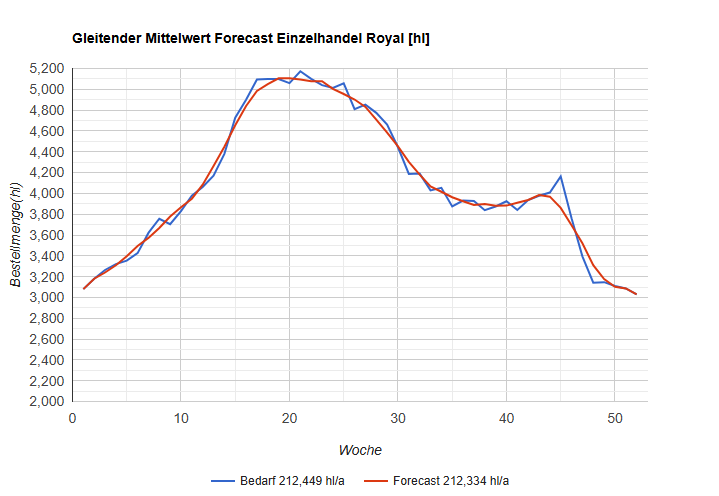
\includegraphics[width=0.7\textwidth]{abbildungen/scm2/scm2forecastperiodewoche5.png}
%    \caption{SCM2 Forecast mit n = 5}
%    \label{fig:SCM2 Forecast mit n = 5}
%\end{figure}
Wie man der Abbildung \ref{fig:SCM2 Forecast mit n = 5} entnehmen kann,
stellt die rote Linie den Forecast dar, während die blaue Linie den tatsächlichen Bedarf zeigt.
Es ist deutlich zu erkennen, dass der Forecast sehr eng am tatsächlichen Bedarf liegt und sich ab etwa Woche 15 gut an die saisonalen Schwankungen anpasst, einschließlich des saisonalen Rückgangs.

Zudem wird sichtbar, dass Ausreißer, insbesondere im Zeitraum von Woche 45 bis etwa Woche 50, geglättet werden und der Forecast weiterhin dem tatsächlichen Bedarf eng folgt.

%\subsubsection{Optimierung der Bestellkosten im Einzelhandel}

\subsubsection{Umgang mit Lieferverzögerungen über Blockchain \& Smart Contracts}
Die Verwendung von Blockchain und Smart Contracts ist ein wichtiges Thema im Supply Chain Management.
Die Funktion der Blockchain besteht darin, eine Kette spezieller Datensätze in einer dezentralen Datenbank zu speichern.
Jeder dieser Blöcke enthält einen kryptographischen Hash sowie zusätzlich den Hash des vorherigen Blocks, wodurch eine unveränderbare und nachvollziehbare Kette entsteht.

Smart Contracts stellen eine ergänzende Komponente der Blockchain-Technologie dar.
Sie ermöglichen die Automatisierung von Aufgaben innerhalb der Lieferkette, etwa die automatische Auslösung einer Zahlung beim Wareneingang eines Produkts.
Ein Smart Contract ist ein digitaler Vertrag in Form von Computercode, der auf der Blockchain gespeichert und für alle Beteiligten einsehbar ist.

Trotz der Automatisierung durch Smart Contracts ist eine sorgfältige Prüfung der Abläufe notwendig Due Diligence,
um die Korrektheit und Verlässlichkeit der Prozesse sicherzustellen.

Das Planspiel bot nur begrenzte Möglichkeiten, die Blockchain-Technologie realitätsnah darzustellen.
Einzig durch die simulierten Lieferverzögerungen ließ sich ansatzweise nachvollziehen, wie eine verbesserte Transparenz durch Blockchain zur Risikominimierung beitragen könnte.

Dennoch wurde im Planspiel deutlich, wie wichtig Technologien wie Blockchain sind, um potenzielle Risiken frühzeitig zu erkennen und präventiv zu handeln.
Im konkreten Fall konnten auf die Lieferverzögerungen wurden geeigneten Maßnahmen ergriffen,
da zu spät erkannt wurde, was mit diesen Verzögerungen konkret gemeint war und welche Auswirkungen sie auf die Lieferkette haben würden.
\subsubsection{Anwendung des Kanban-Prinzips zur Optimierung der Lieferkette}
Kanban wurde von Taiichi Ohno, einem Ingenieur bei Toyota, entwickelt und stellt ein zentrales Konzept im Lean Management dar.
Das Hauptziel von Kanban ist die Umsetzung des Just-in-Time-Prinzips, um den Lagerbestand innerhalb eines Produktionssystems zu minimieren.

Das Grundprinzip besteht darin, dass eine Karte (Kanban) existiert, die in einer festgelegten Reihenfolge verschiedene Produktionsstationen durchläuft.
Diese Karte wird nur dann an die nächste Station weitergegeben, wenn der Produktionsschritt an der aktuellen Station abgeschlossen ist.
Gleichzeitig wird sie an die vorherige Station zurückgegeben, um dort den nächsten Produktionsvorgang auszulösen.
Dieser Zyklus wiederholt sich so lange, bis das Endprodukt vollständig gefertigt ist. --Quelle--

Dieses Prinzip könnte auch im Planspiel Anwendung finden, um die Effizienz der Bestellprozesse zu steigern.
Die Umsetzung würde so gestaltet, dass Bestellungen den Weg von links nach rechts durchlaufen, also vom Einzelhandel bis zur Materialbeschaffung.
Dabei spielt die Kommunikation zwischen den Geschäftsbereichen eine entscheidende Rolle,
um die Lagerbestände möglichst gering zu halten und gleichzeitig Engpässe zu vermeiden.

Wichtig ist dennoch anzumerken, dass das Prinzip des Kanban theoretisch im Planspiel angewendet wird,
indem die Geschäftsbereiche nur ihre Bestellungen aufgeben und somit die Kanban-Karte von 
einem Geschäftsbereich zum nächsten weitergegeben wird,
wenn die Bestellung ausgelöst wird. Es fehlt jedoch die Kalkulierung der Lagerbestände, um diese minimieren zu können.
\newpage
\subsection{Spielrunde 3 – CRM2: Kundenmanagement mit Big Data}
Wie bereits in der Einleitung erwähnt, wurde in der dritten Spielrunde (CRM2) das Customer Relationship Management simuliert.
In dieser Runde agierten die Teammitglieder nicht als Geschäftsbereiche, sondern als Einzelhändler. 
Einzelhändler 1, bestehend aus zwei Teammitgliedern, musste dabei zwölf Produkte aufteilen.

Ziel dieser Runde war es, durch gezielte Vermarktung der Produkte sowohl den Umsatz als auch das Wachstum zu steigern. 
Anders als in den vorherigen Runden traten die Unternehmen nicht direkt gegeneinander an,
stattdessen konkurrierten die Einzelhändler untereinander,
während das Unternehmen als Gesamtheit weiterhin als eine geschlossene Einheit fungierte.
Es wurden insgesamt 12 Spielrunden gespielt, die jeweils 4 Wochen also 1 Monat repräsentierten.
\subsubsection{Analyse der Einzelhandel eins Ergebniss}
%\begin{table}[H]
%    \centering
%    \resizebox{\textwidth}{!}{ 
%    \csvautotabular[separator=semicolon]{tabellen/crm2/produkte.csv}}
%    \caption{CRM 2 Produktliste}
%    \label{tab:CRM 2 Produktliste}
%\end{table}
Die Tabelle zeigt die Produkte, die dem Einzelhandel 1 zugeordnet wurden.
In der ersten Spielrunde musste entschieden werden, welche Produkte beworben werden sollten.
Nach gemeinsamer Teamentscheidung wurde beschlossen, dass der Bügel-Kasten und der Premium-Kasten nicht beworben werden,
was sich im Nachhinein als folgenschwere Entscheidung herausstellte.
Das Unternehmen Alpha hat diese beiden Produkte als einziges Unternehmen beworben und konnte somit ein Monopol aufbauen.

Gleichzeitig gelang es jedoch, für die Produkte Premium-Flasche,
Premium-12er-Pack und Alkoholfrei-Kasten ein Monopol für Royal aufzubauen.
Diese drei Produkte wurden bis zur sechsten Spielrunde kontinuierlich vermarktet,
um den Umsatz so weit wie möglich zu steigern.
Zusätzlich wurde auf konkurrierende Produkte ein- bis zweimal ein Rabatt angewendet,
um deren Umsatzwachstum gezielt zu unterbrechen.

Während der Saison wurde auf Werbung verzichtet.
Stattdessen wurde jeweils einmal der Preis erhöht,
um den Umsatz zu maximieren und gleichzeitig den anderen Einzelhändlern im Unternehmen Royal zu ermöglichen,
sich auf ihre starken Produkte zu konzentrieren.
Nach der Saison wurde zum Abschluss nochmals Werbung geschaltet, um den positiven Saison-Effekt mitzunehmen.

Um den Effekt der Vermarktung zu verdeutlichen, wurden die Umsätze vom Royal, 
Green und Wild für das Produkt Premium-Flasche in Abbildung dargestellt.
%\begin{figure}[H]
%    \centering
%    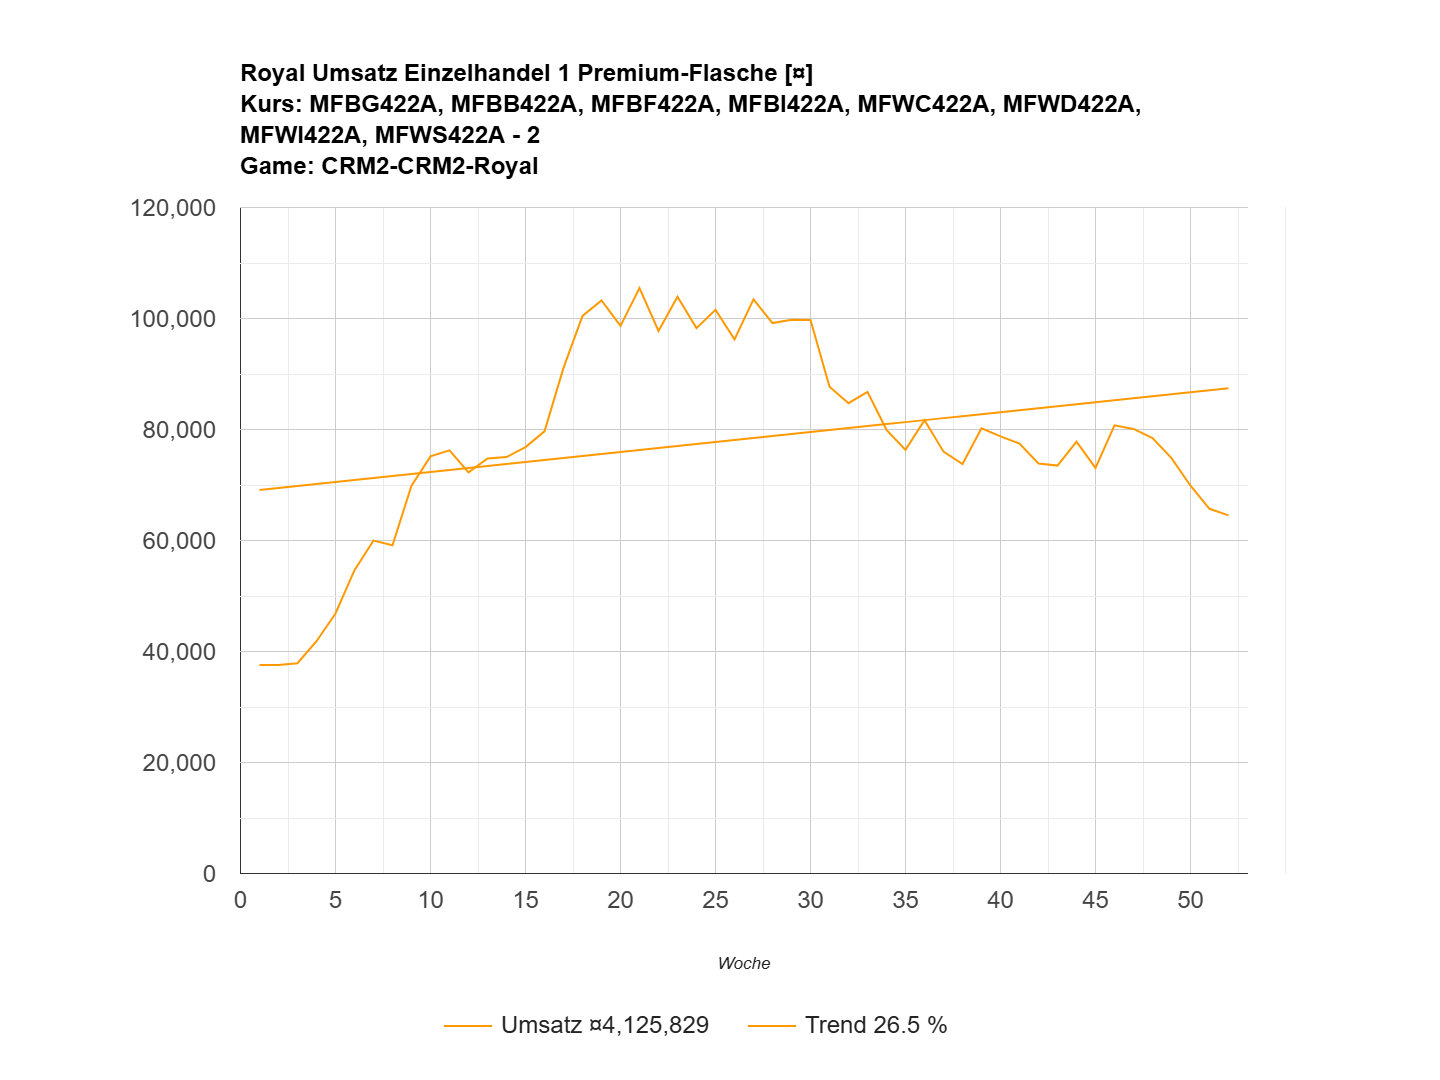
\includegraphics[width=0.7\textwidth]{abbildungen/crm2/Royal-Premiumflasche.png}
%    \caption{Royal Premium-Flasche}
%    \label{fig:Royal Premium-Flasche}
%\end{figure}
Wie oben beschrieben, wurde für das Produkt Premium-Flasche in den ersten zehn Wochen aktiv Marketing betrieben. 
Dadurch konnte der Umsatz auf durchschnittlich etwa 65.000 Euro gesteigert werden.
Durch die Saison sowie eine gezielte Preiserhöhung stieg der Umsatz zeitweise auf rund 100.000 Euro an.
Nach der Saison wurde erneut Werbung geschaltet, um den Saison-Effekt mitzunehmen.
Dies führte dazu, dass der durchschnittliche Umsatz von Woche 33 bis 50 bei etwa 75.000 Euro lag.
%\begin{figure}[H]
%    \centering
%    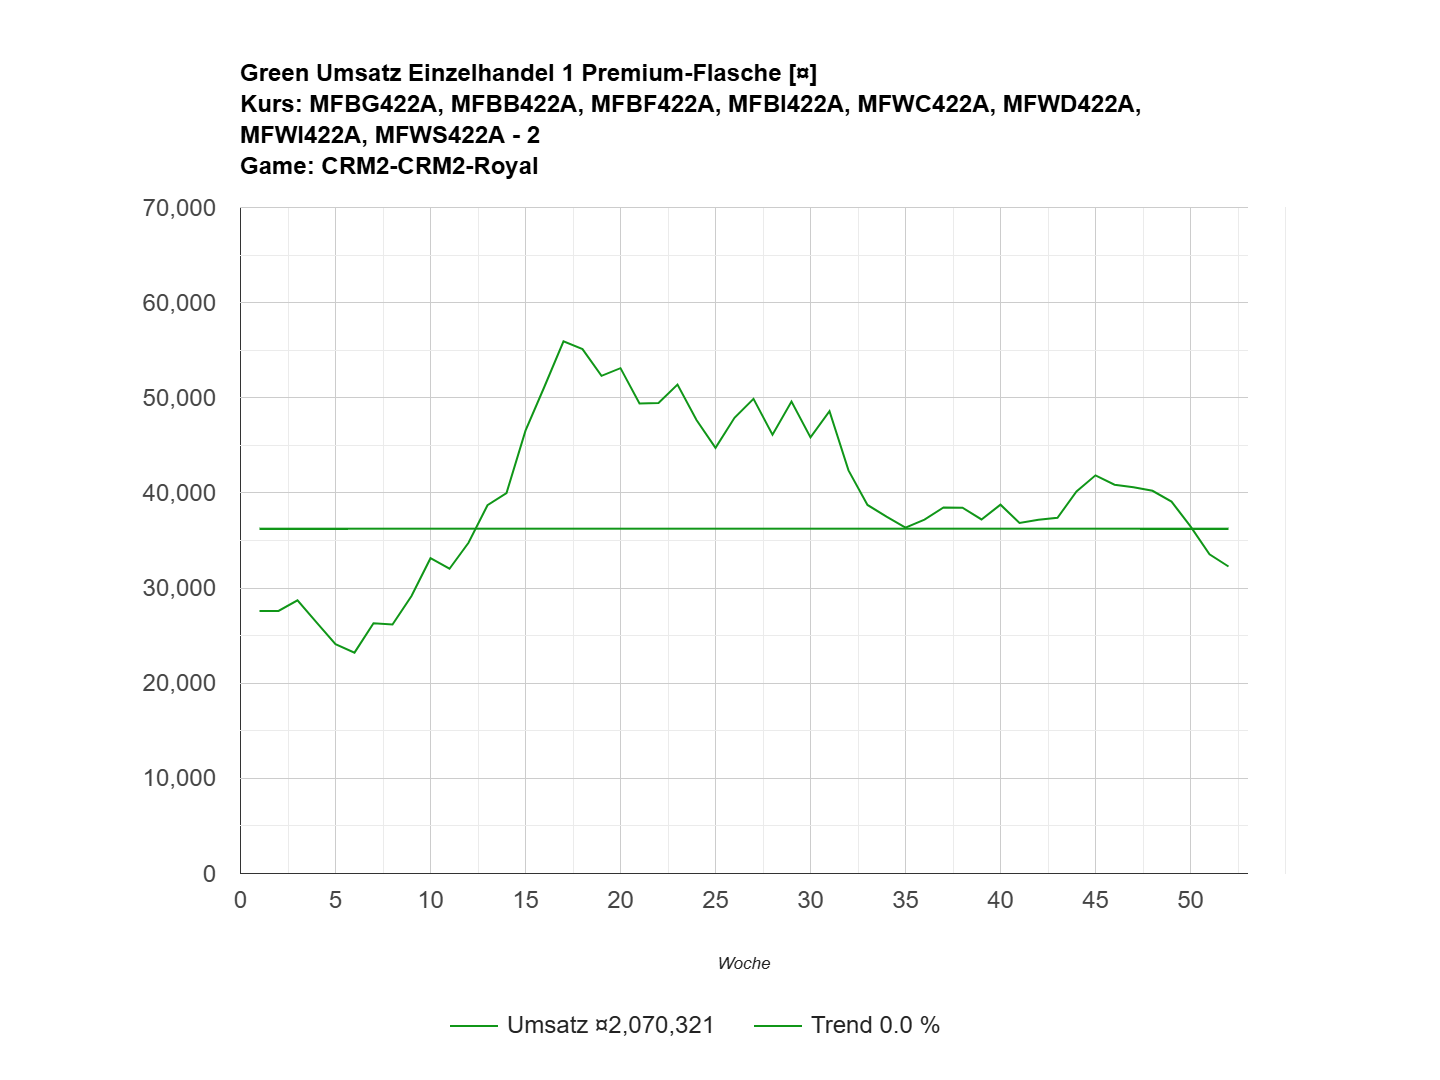
\includegraphics[width=0.7\textwidth]{abbildungen/crm2/green-Premiumflasche.png}
%    \caption{Green Premium-Flasche}
%    \label{fig:Green Premium-Flasche}
%\end{figure}
Wie in Abbildung \ref{fig:Green Premium-Flasche} zu sehen ist, wurde das Produkt Premium-Flasche von Green ebenfalls angeboten, 
jedoch ohne den Einsatz von Marketingmaßnahmen.
Stattdessen wurde lediglich der Preis gesenkt, um im Markt konkurrenzfähig zu bleiben.
Dennoch zeigt sich ein deutlicher Unterschied im Umsatz zwischen Green und Royal,
da Royal durch gezielte Marketingmaßnahmen den Umsatz nahezu verdoppeln konnte.
%\begin{figure}[H]
%    \centering
%    \includegraphics[width=0.7\textwidth]{abbildungen/crm2/wild-Premiumflasche.png}
%    \caption{Wild Premium-Flasche}
%    \label{fig:Wild Premium-Flasche}
%\end{figure}
Der Unterschied zwischen Wild und den Unternehmen Royal und Green ist enorm, da Wild das Produkt zwar beworben hat,
jedoch keine weiteren Maßnahmen ergriff, um den Umsatz stabil zu halten.
Dementsprechend sank der Umsatz von etwa 30.000 Euro auf rund 18.000 Euro.
Zwar ist ein saisonaler Effekt erkennbar, jedoch zeigt der Umsatzverlauf von Wild, dass es nicht gelungen ist,
den durchschnittlichen Umsatz von ca. 30.000 Euro nachhaltig zu erreichen.
Stattdessen konnte der Umsatz lediglich während der Saison stabil gehalten werden,
bevor er sich nach deren Ende dauerhaft bei etwa 18.000 Euro einpendelte.

\subsubsection{Performance-Analyse mit Word Tree \& beworbenen Produkten}
%\begin{figure}[H]
%    \centering
%    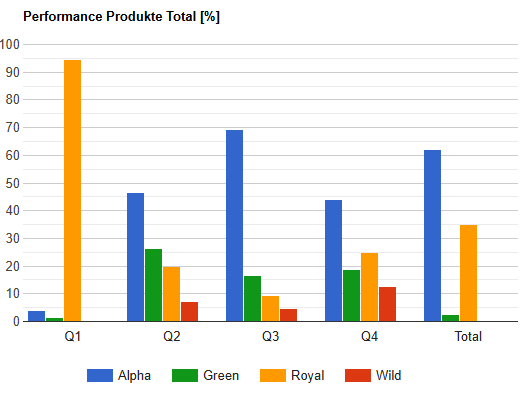
\includegraphics[width=0.7\textwidth]{abbildungen/crm2/Performance.png}
%    \caption{Performance Total}
%    \label{fig:Performance Total}
%\end{figure}
Auch im Bereich der Performance-Analyse spiegeln die Ergebnisse die zuvor beschriebenen Beobachtungen wider.
Es wird deutlich, dass im ersten Quartal ein Großteil des Budgets ausgegeben wurde.
Das hatte zur Folge, dass in den folgenden Quartalen kaum noch Budget zur Verfügung stand,
um Produkte weiterhin zu vermarkten, Preisnachlässe zu gewähren oder Preiserhöhungen vorzunehmen.
Dadurch sank die Performance in den späteren Quartalen drastisch und konnte nicht mehr vollständig ausgeschöpft werden.

Im Vergleich dazu war die Strategie von Alpha besser,
da dort von Quartal zwei bis Quartal vier die Performance weitgehend konstant gehalten wurde.
Das bedeutet, dass Royal von den anfänglich erreichten 94\% Performance etwa 50\% hätte reduzieren und stattdessen gleichmäßig
auf die Quartale zwei bis vier verteilen sollen, um eine konstante Performance zu erzielen.
Dies würde auch erklären, warum Royal insgesamt nur rund 35\% der Gesamtperformance erreicht hat,
während Alpha etwa 60\% erzielen konnte.

%\begin{figure}[H]
%    \centering
%    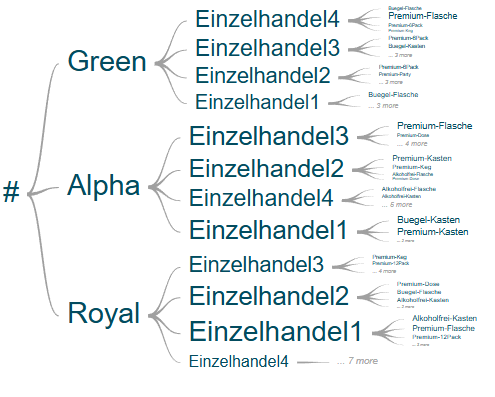
\includegraphics[width=0.7\textwidth]{abbildungen/crm2/World-Tree.png}
%    \caption{Performance Total}
%    \label{fig:Performance Total}
%\end{figure}

Die World Tree-Analyse zeigt, dass die Produkte Alkoholfrei-Kasten,
Premium-Flasche und Premium-12er-Pack die besten Ergebnisse für Royal erzielt haben.
Die Marktpräsenz von Einzelhandel 1 des Unternehmens Royal ist dabei deutlich höher als die der
Mitbewerber Green und Wild. Es ist erkennbar,
dass diese drei Produkte fast die gleiche Gewichtung haben und sich daher sehr
stark im Markt präsentieren konnten.

Im Vergleich dazu war von Alpha lediglich zwei Produkte stärker auf dem Markt vertreten.
Obwohl einige Einzelhändler von Royal in bestimmten Bereichen stärker vertreten waren,
bleibt Alpha insgesamt der stärkere Akteur auf dem Markt.

%\subsubsection{Einsatz von Sentiment Analysis im CRM und Marketing}

\newpage
% Fazit
\section{Fazit}
Insgesamt stellt die Simulation eine lehrreiche Erfahrung dar,
die verdeutlicht, welche Geschäftsprozesse und Themen entscheidend sind,
um eine Supply Chain effizient zu gestalten und ein erfolgreiches Customer Relationship Management
zu betreiben. Sie zeigt auf, welche Grundlagen geschaffen werden müssen,
um eine funktionierende Supply Chain überhaupt anwenden zu können.

Wie insbesondere in den ersten beiden Spielrunden deutlich wurde,
spielen Kommunikation, Forecasting und Blockchain-Technologie eine zentrale Rolle,
um eine vorausschauende Steuerung der Lieferkette zu ermöglichen und auf Risiken reagieren zu können,
ohne dass diese gravierende Auswirkungen auf das Unternehmen haben. Zudem wurde deutlich,
dass emotionale Entscheidungen zu Verlusten führen können,
die sich in Form von hohen Lagerkosten oder Fehlmengenkosten niederschlagen.
Durch den Einsatz von Forecast-Methoden und rationalen Entscheidungen können diese Kosten deutlich
reduziert oder zumindest kalkulatorisch eingeplant werden.

Auch im Bereich des Customer Relationship Managements wurde sichtbar,
dass Produkte, die nicht aktiv beworben werden, dennoch sinnvoll im Produktportfolio verbleiben können,
um passiven Umsatz zu generieren. Ebenso ist es essenziell,
das vorhandene Marketingbudget gleichmäßig über die Quartale zu verteilen,
um eine konstante und möglichst hohe Performance über den gesamten Zeitraum zu erzielen.
% Literaturverzeichnis
\newpage
\addcontentsline{toc}{section}{Literaturverzeichnis}
\section*{Literaturverzeichnis}
\begin{thebibliography}{99}
    \bibitem{Gronwald2020} Gronwald, (2020). \textit{Integrierte Business-Informationssysteme – Ganzheitliche, geschäftsprozessorientierte Sicht auf die vernetzte Unternehmensprozesskette ERP, SCM, CRM, BI, Big Data Analytics}. Springer Vieweg, 2020. Verfügbar unter: \url{https://link.springer.com/book/10.1007/978-3-662-59815-3} (zuletzt aufgerufen am 27.04.2025)
    \bibitem{Kdibisglobal} Gronwald, K.D. \textit{kdibisglobal – Planspiel zur Umsetzung integrierter Business-Informationssysteme}. Verfügbar unter: \url{https://www.kdibisglobal.org/php/kdiglobstart.php} (zuletzt aufgerufen am 27.04.2025)
\end{thebibliography}


\newpage
% Anhang
%\appendix
%\section{Anhang}
%Hier können zusätzliche Informationen, wie Code-Beispiele oder ausführliche Tabellen, eingefügt werden.

% Ehrenwörtliche Erklärung
\newpage
\addcontentsline{toc}{section}{Ehrenwörtliche Erklärung}
\section*{\texttt{Ehrenwörtliche Erklärung}}
Hiermit erkläre ich, dass ich die vorliegende schriftliche Ausarbeitung im Modul \textbf{Implementierung digitaler Geschäftsprozesse} selbstständig
angefertigt habe. Es wurden nur die in der Arbeit ausdrücklich benannten Quellen und
Hilfsmittel benutzt. Wörtlich oder sinngemäß übernommenes Gedankengut habe ich als
solches kenntlich gemacht. Diese Arbeit hat in gleicher oder ähnlicher Form noch keiner
Prüfungsbehörde vorgelegen.

\vspace{3cm}
\noindent\begin{tabular}{p{0.5\textwidth}p{0.5\textwidth}}
    \hrulefill & \hrulefill \\
    Ort, Datum & Unterschrift \\
\end{tabular}

\end{document}
